\section{Participación multidimensional del egresado}

La participación de un egresado no se reduce a una sola huella. Una misma persona puede contratar con el Estado, registrar una empresa y figurar como investigadora reconocida, y hasta ahora cada una de esas huellas se observaba por separado, en fuentes distintas y sin un punto de cruce común. Esta sección reúne las tres dimensiones ---contratación pública (SECOP), actividad empresarial (RUES) y trayectoria investigativa (CvLAC)--- sobre una base de 174.685 graduados de las seis sedes de la Universidad Santo Tomás, consolidadas por cédula. El resultado es una lectura del egresado como un actor que deja, con frecuencia, más de una marca verificable en el país, y que permite preguntarse no solo cuántos dejan huella, sino con qué intensidad, desde qué nivel de formación, en qué sede y en qué combinación.

\subsection{Una tabla por persona}

El informe previo dejó pendiente justamente este paso, el de pasar de contar registros a contar personas. Un mismo graduado podía aparecer varias veces en SECOP, varias en RUES y de nuevo en CvLAC, de modo que sumar registros sobreestimaba el alcance real. Al consolidar las tres fuentes por cédula, cada graduado ocupa una sola fila y se le asocia el número de dimensiones en las que deja huella, de cero a tres. De los 174.685 graduados, 104.308 no registran huella en ninguna de las tres fuentes públicas consultadas, mientras que 70.377 aparecen al menos en una, como detalla la Tabla~\ref{tab:dist-dimensiones} y resume la Figura~\ref{fig:dimensiones}.

\begin{table}[H]
\centering
\caption{Distribución de graduados según el número de dimensiones de participación.}
\label{tab:dist-dimensiones}
\begin{tabularx}{0.78\linewidth}{Xrr}
\toprule
\rowcolor{ustaazul}\textbf{\color{white}Número de dimensiones} & \textbf{\color{white}Graduados} & \textbf{\color{white}Porcentaje} \\
\midrule
Ninguna (0) & 104.308 & 59,7\,\% \\
Una (1) & 58.001 & 33,2\,\% \\
Dos (2) & 12.149 & 7,0\,\% \\
Las tres (3) & 227 & 0,1\,\% \\
\midrule
\textbf{Total} & \textbf{174.685} & \textbf{100,0\,\%} \\
\bottomrule
\end{tabularx}
\end{table}

\begin{figure}[H]\centering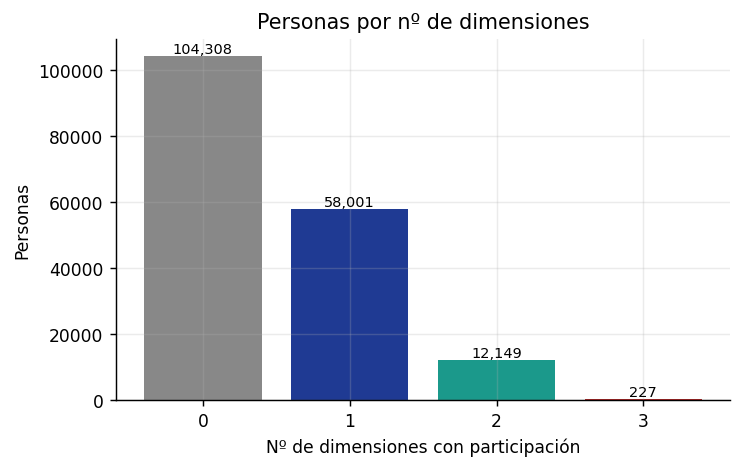
\includegraphics[width=0.78\linewidth]{figs_cruce/06_dimensiones.png}\caption{Distribución de graduados por número de dimensiones de participación.}\label{fig:dimensiones}\end{figure}

La lectura conviene hacerla con una cautela metodológica de fondo. Que seis de cada diez graduados no aparezcan en ninguna fuente no significa que carezcan de participación, sino que su trayectoria ---el empleo asalariado en el sector privado, el ejercicio liberal sin contratación estatal, la docencia, la migración al exterior--- transcurre por canales que estos tres registros públicos no capturan. Lo que el cruce mide no es, por tanto, la participación total del egresado, sino su huella en tres dominios concretos y verificables. Dentro de esos límites, la cifra es contundente.

\begin{cajahallazgo}
Cuatro de cada diez graduados (40,3\,\%) dejan huella verificable en al menos una de las tres dimensiones de participación, ya sea porque contratan con el Estado, porque se registran en el RUES o porque investigan. Es la primera vez que esta cifra se mide sobre la persona y no sobre el registro, lo que la convierte en una línea de base sólida para el seguimiento de los próximos años.
\end{cajahallazgo}

\subsection{Las combinaciones de participación}

Más allá del recuento por número de dimensiones, interesa saber qué facetas específicas se combinan en cada graduado, pues no es lo mismo contratar y registrarse en el RUES que investigar y contratar. La Tabla~\ref{tab:combinaciones} y la Figura~\ref{fig:combinaciones} descomponen los perfiles de quienes tienen al menos una huella.

\begin{table}[H]
\centering
\caption{Combinaciones de dimensiones entre los graduados con al menos una huella.}
\label{tab:combinaciones}
\begin{tabularx}{0.74\linewidth}{Xrr}
\toprule
\rowcolor{ustaazul}\textbf{\color{white}Combinación} & \textbf{\color{white}Graduados} & \textbf{\color{white}\%} \\
\midrule
Solo SECOP & 30.790 & 43,7\,\% \\
Solo RUES & 25.815 & 36,7\,\% \\
SECOP + RUES & 11.225 & 16,0\,\% \\
Solo CvLAC & 1.396 & 2,0\,\% \\
SECOP + CvLAC & 647 & 0,9\,\% \\
RUES + CvLAC & 277 & 0,4\,\% \\
SECOP + RUES + CvLAC & 227 & 0,3\,\% \\
\bottomrule
\end{tabularx}
\end{table}

\begin{figure}[H]\centering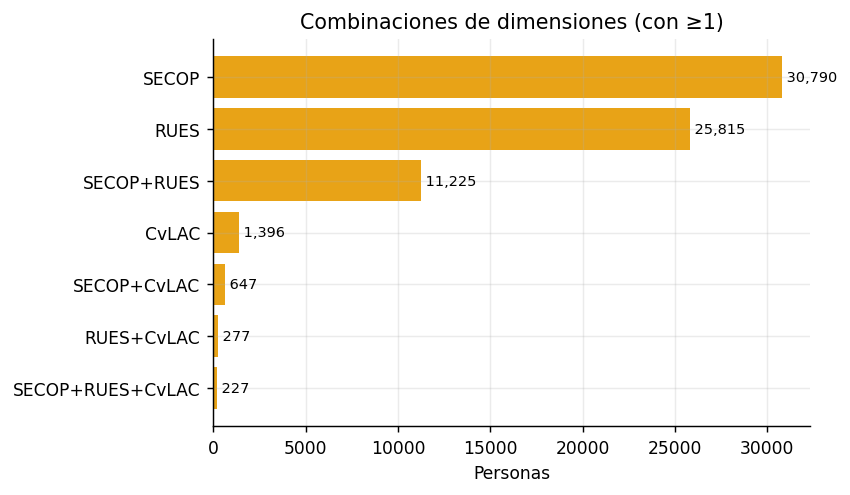
\includegraphics[width=0.78\linewidth]{figs_cruce/07_combinaciones.png}\caption{Combinaciones de participación entre los graduados que registran al menos una huella.}\label{fig:combinaciones}\end{figure}

Las huellas individuales dominan el panorama: la contratación pública en solitario reúne a 30.790 graduados (el 43,7\,\% de quienes dejan huella) y el registro empresarial en solitario a 25.815 (36,7\,\%). La combinación doble más frecuente es SECOP\,+\,RUES, con 11.225 graduados que a la vez contratan con el Estado y registran empresa, una cercanía natural porque muchos contratistas operan a través de compañías propias y comparten un mismo motor de actividad económica formal. Las combinaciones que incluyen investigación, en cambio, son marginales: 647 graduados suman SECOP y CvLAC, 277 reúnen RUES y CvLAC y solo 227 las tres dimensiones. La rareza de los perfiles con CvLAC confirma que la investigación reconocida es la más exigente y la menos extendida de las tres facetas.

\subsection{La intensidad de la huella}

Aparecer en una fuente y aparecer con fuerza son cosas distintas. Para matizar el recuento conviene mirar \emph{cuánta} huella deja quien deja huella, y el panorama es el de una amplia base de participación ligera coronada por una cola muy larga. La mediana del proveedor del Estado es de \textbf{5 contratos}, aunque el promedio sube a 8 por efecto de unos pocos contratistas con cientos de vínculos; la del matriculado en el RUES es de \textbf{una sola matrícula} mercantil; y la del investigador, de \textbf{2 productos} registrados, con un promedio de 5,7 que delata la presencia de unos cuantos investigadores muy prolíficos. En las tres dimensiones, por tanto, la norma es la huella modesta ---un puñado de contratos, una empresa, un par de publicaciones--- y la excepción son los perfiles intensivos que concentran la mayor parte del volumen. Esa asimetría, ya señalada en el capítulo de contratación a propósito de los megacontratos, recomienda leer la participación en términos de \emph{cuántas personas} participan antes que de los agregados, siempre dominados por los extremos.

\subsection{Participación y nivel de formación}

¿Pesa el posgrado en la huella del egresado? El cruce con la modalidad de formación ---disponible para los graduados de todas las sedes--- responde de forma afirmativa y nítida (Tabla~\ref{tab:modalidad-participación}). El graduado de posgrado deja huella en al menos una dimensión en el \textbf{43,9\,\%} de los casos, frente al \textbf{38,7\,\%} del graduado de pregrado, y la brecha se ensancha en la contratación pública, donde el posgrado alcanza el 30,5\,\% contra el 21,9\,\% del pregrado. También es más frecuente entre los posgraduados el perfil multidimensional, con un 8,8\,\% en dos o más dimensiones frente al 6,3\,\% del pregrado. La matrícula mercantil, en cambio, es prácticamente idéntica en ambos niveles, lo que sugiere que crear empresa depende menos del título y más de la iniciativa individual. La formación avanzada abre, sobre todo, las puertas de la contratación especializada con el Estado y de la investigación, las dos dimensiones donde la credencial posgradual rinde mayores frutos.

\begin{table}[H]
\centering
\caption{Tasas de participación según el nivel de formación (todas las sedes).}
\label{tab:modalidad-participación}
\begin{tabularx}{0.92\linewidth}{Xrrrrr}
\toprule
\rowcolor{ustaazul}\textbf{\color{white}Modalidad} & \textbf{\color{white}Graduados} & \textbf{\color{white}SECOP} & \textbf{\color{white}RUES} & \textbf{\color{white}CvLAC} & \textbf{\color{white}$\geq$1 dim.} \\
\midrule
Pregrado & 120.242 & 21,9\,\% & 21,9\,\% & 1,3\,\% & 38,7\,\% \\
Posgrado & 54.443 & 30,5\,\% & 20,6\,\% & 1,7\,\% & 43,9\,\% \\
\bottomrule
\end{tabularx}
\end{table}

\subsection{Participación por sede}

La participación tampoco se reparte por igual entre las sedes. La Tabla~\ref{tab:tasas-sede} compara las tasas por dimensión y dibuja perfiles diferenciados. Tunja encabeza la contratación pública, con el 45,2\,\% de sus graduados en SECOP, y también la investigación, con el 2,5\,\% en CvLAC, la tasa más alta del sistema; Villavicencio la sigue de cerca en contratación (38,0\,\%), lo que confirma el peso de las sedes regionales en el vínculo con el Estado. Bucaramanga lidera el registro empresarial (29,0\,\% en RUES). Bogotá, con más de cien mil graduados, presenta las tasas relativas más bajas en contratación y matrícula mercantil, un contraste que separa el volumen absoluto de la intensidad de la participación.

\begin{table}[H]
\centering
\caption{Tasas de participación por sede y dimensión.}
\label{tab:tasas-sede}
\begin{tabularx}{0.90\linewidth}{Xrrrr}
\toprule
\rowcolor{ustaazul}\textbf{\color{white}Sede} & \textbf{\color{white}Graduados} & \textbf{\color{white}SECOP} & \textbf{\color{white}RUES} & \textbf{\color{white}CvLAC} \\
\midrule
Bogotá & 104.468 & 20,0\,\% & 18,2\,\% & 1,5\,\% \\
Bucaramanga & 36.554 & 28,2\,\% & 29,0\,\% & 1,3\,\% \\
Tunja & 13.803 & 45,2\,\% & 24,8\,\% & 2,5\,\% \\
Villavicencio & 6.697 & 38,0\,\% & 24,2\,\% & 1,2\,\% \\
Medellín & 2.936 & 28,9\,\% & 17,8\,\% & 1,1\,\% \\
VUAD & 10.227 & 19,9\,\% & 23,3\,\% & 0,6\,\% \\
\bottomrule
\end{tabularx}
\\[2pt]{\scriptsize\color{ustagris} Aquí cada persona se asigna a una sola sede (su sede principal), de modo que los totales suman las 174.685 personas únicas. Difieren de la Tabla~\ref{tab:base_unificada}, que cuenta a quien tiene título en varias sedes dentro de cada una.}
\end{table}

\begin{figure}[H]\centering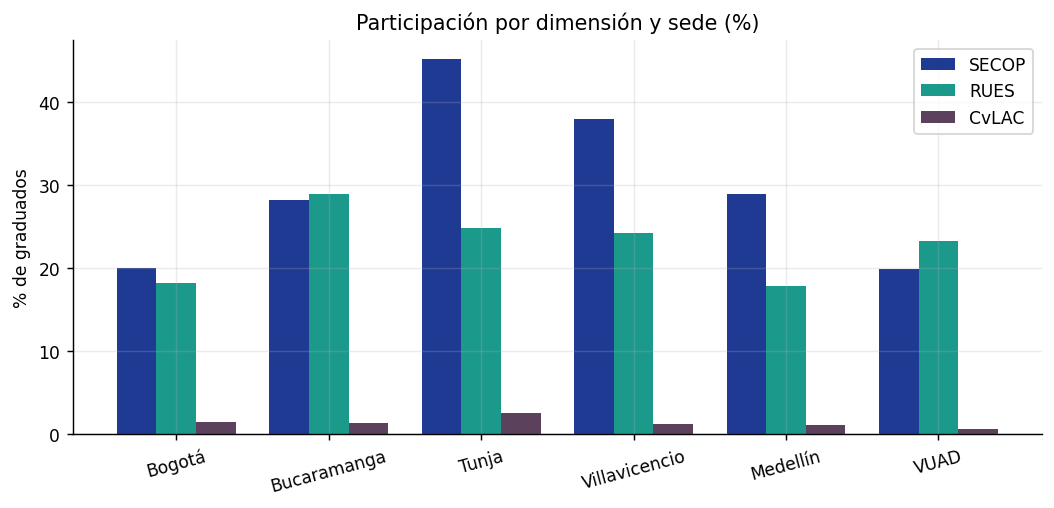
\includegraphics[width=0.80\linewidth]{figs_cruce/05_tasas_seccional.png}\caption{Tasa de graduados con huella por dimensión y sede.}\label{fig:tasas-seccional}\end{figure}

La composición por número de dimensiones (Figura~\ref{fig:dimensiones-seccional}) refuerza la lectura desde el ángulo de la acumulación. Tunja es la única sede donde los graduados con al menos una huella superan a quienes no tienen ninguna, y también la que concentra la mayor proporción de perfiles multidimensionales: el \textbf{14,2\,\%} de sus egresados deja huella en dos o más dimensiones, frente al 11,1\,\% de Villavicencio, el 9,2\,\% de Bucaramanga y apenas el 5,1\,\% de Bogotá. La geografía de la participación del egresado tomasino es, por tanto, desigual no solo en su frecuencia sino en su densidad, y conviene leerla siempre en proporciones antes que en conteos absolutos, dado el enorme peso numérico de la sede principal.

\begin{figure}[H]\centering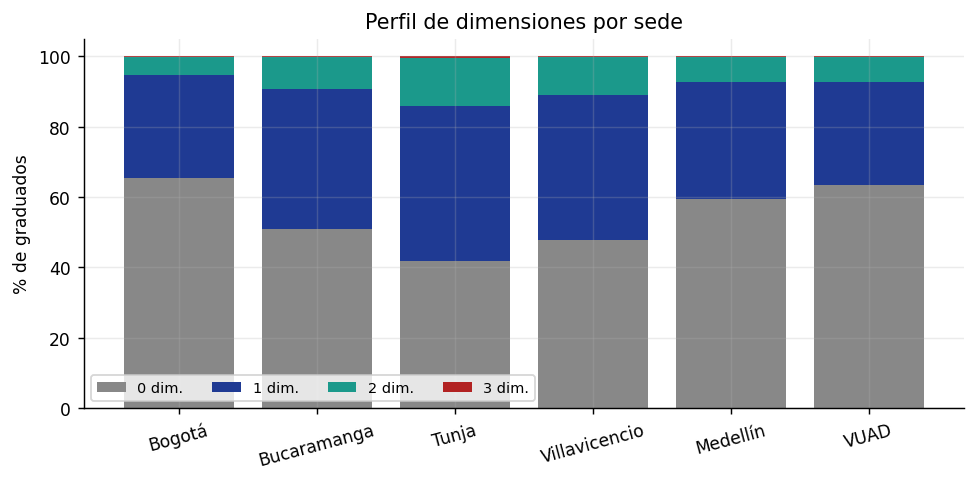
\includegraphics[width=0.80\linewidth]{figs_cruce/08_dimensiones_seccional.png}\caption{Perfil de graduados por número de dimensiones de participación (de cero a tres) en cada sede.}\label{fig:dimensiones-seccional}\end{figure}

\subsection{Participación según la cohorte de graduación}

La huella de un egresado se acumula con el tiempo, de modo que la participación por década de graduación debe leerse con cautela. La Tabla~\ref{tab:participación-decada} y la Figura~\ref{fig:participación-cohorte} muestran cómo la contratación pública crece de forma sostenida desde los años noventa hasta su máximo en la cohorte de 2010 (33,8\,\%), para descender al 28,6\,\% en la de 2020.

\begin{table}[H]
\centering
\caption{Tasas de participación según la década de graduación.}
\label{tab:participación-decada}
\begin{tabularx}{0.92\linewidth}{Xrrrr}
\toprule
\rowcolor{ustaazul}\textbf{\color{white}Década} & \textbf{\color{white}Graduados} & \textbf{\color{white}SECOP} & \textbf{\color{white}RUES} & \textbf{\color{white}CvLAC} \\
\midrule
1970 & 1.104 & 8,3\,\% & 27,4\,\% & 0,8\,\% \\
1980 & 9.355 & 11,1\,\% & 25,0\,\% & 0,8\,\% \\
1990 & 36.996 & 11,0\,\% & 22,4\,\% & 0,7\,\% \\
2000 & 35.939 & 24,9\,\% & 24,9\,\% & 1,6\,\% \\
2010 & 50.780 & 33,8\,\% & 21,9\,\% & 2,6\,\% \\
2020 & 40.490 & 28,6\,\% & 16,1\,\% & 0,8\,\% \\
\bottomrule
\end{tabularx}
\end{table}

\begin{figure}[H]\centering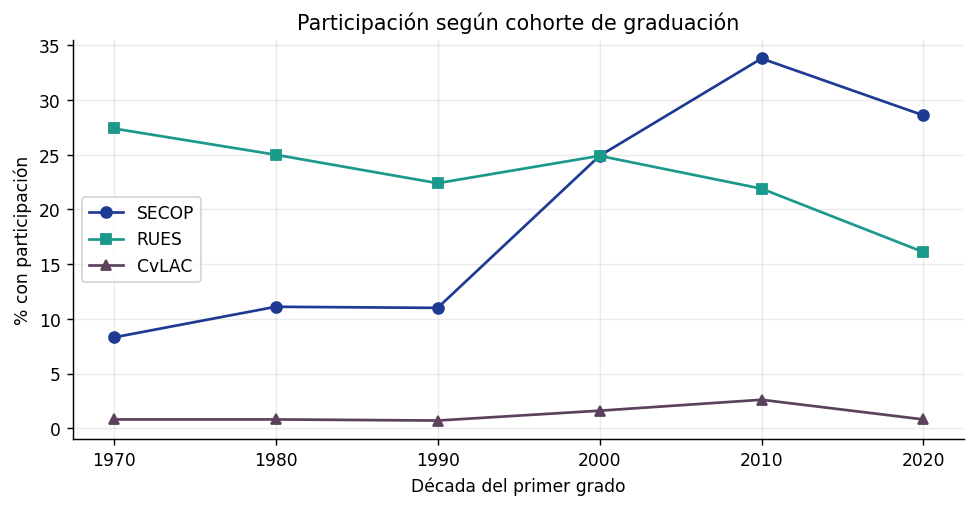
\includegraphics[width=0.80\linewidth]{figs_cruce/09_impacto_cohorte.png}\caption{Tasas de participación por dimensión según la década de graduación.}\label{fig:participación-cohorte}\end{figure}

La trayectoria investigativa sigue un patrón parecido al de la contratación, con su pico también en 2010 (2,6\,\%), mientras que el registro empresarial es más estable y cede algo en la cohorte más reciente. Dos factores explican esta forma. Por un lado, las cohortes recientes han tenido menos años para dejar huella, así que su menor tasa refleja exposición y no necesariamente potencial. Por otro, la cobertura del SECOP arranca a mediados de la década de 2000, lo que deprime artificialmente las tasas de contratación de las cohortes más antiguas, cuyos contratos previos no quedaron registrados en la plataforma. La caída de la cohorte de 2020 no debe interpretarse, por todo ello, como una pérdida de participación, sino como una maduración aún incompleta que solo los seguimientos de los próximos años podrán medir.

\subsection{El núcleo multidimensional}

El cruce por cédula permite, por fin, mirar de cerca a quienes concentran varias formas de participación a la vez. El solapamiento más frecuente es el de contratación y matrícula mercantil, con 11.452 graduados que figuran simultáneamente en SECOP y RUES. Pero la asociación más reveladora aparece alrededor de la investigación, la población más pequeña y exigente: entre los graduados con trayectoria en CvLAC, alrededor del \textbf{34,3\,\%} también contrata con el Estado y cerca del \textbf{19,8\,\%} también registra empresa, tasas muy por encima de las de la población egresada en general (Figura~\ref{fig:overlaps}). El investigador tomasino, lejos de ser una figura ensimismada, es con frecuencia un profesional activo que además contrata y se registra en el RUES.

\begin{figure}[H]\centering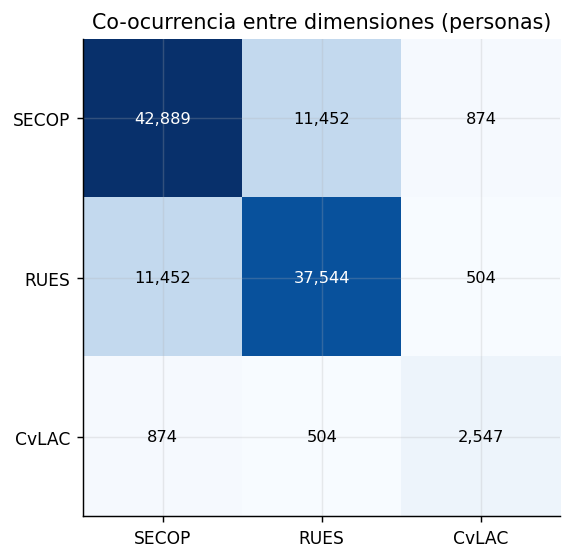
\includegraphics[width=0.62\linewidth]{figs_cruce/15_overlaps.png}\caption{Co-ocurrencia entre las tres dimensiones de participación (número de graduados).}\label{fig:overlaps}\end{figure}

En la cúspide de esa convergencia están los \textbf{227 graduados} que reúnen las tres dimensiones a la vez ---contratan, se registran en el RUES e investigan---, un núcleo diminuto pero significativo que ninguna fuente aislada habría podido identificar. Su distribución no es uniforme: 101 provienen de Bogotá, 60 de Bucaramanga y 49 de Tunja, y los 17 restantes de la VUAD (9), Villavicencio (6) y Medellín (2), de modo que Tunja aporta a este grupo de élite una proporción muy superior a su peso poblacional. Por programa, el Derecho domina con holgura (37 personas), seguido de la Especialización en Derecho Administrativo (14), la Arquitectura (11), la Maestría en Educación (10) y la Economía (9), una mezcla de profesiones liberales clásicas y de posgrados profesionalizantes. Conviene insistir en que toda esta convergencia es de \emph{asociación} y no de causalidad: los datos no permiten afirmar que investigar produzca mayor contratación o matrícula mercantil, sino que las tres facetas tienden a concentrarse en perfiles especialmente activos, formados y conectados.

\subsection{Participación por programa}

El tipo de huella depende, por último, en buena medida del programa cursado, como recoge el mapa de calor de la Figura~\ref{fig:heatmap-programa} y detalla la Tabla~\ref{tab:heatmap-programa}.

\begin{table}[H]
\centering
\caption{Tasas de participación por dimensión en programas seleccionados.}
\label{tab:heatmap-programa}
\begin{tabularx}{0.95\linewidth}{Xrrr}
\toprule
\rowcolor{ustaazul}\textbf{\color{white}Programa} & \textbf{\color{white}SECOP} & \textbf{\color{white}RUES} & \textbf{\color{white}CvLAC} \\
\midrule
Especialización en Derecho Administrativo & 57,7\,\% & 20,4\,\% & 0,8\,\% \\
Derecho & 44,1\,\% & 18,0\,\% & 1,5\,\% \\
Ingeniería Civil & 34,0\,\% & 25,4\,\% & 1,2\,\% \\
Cultura Física, Deporte y Recreación & 31,5\,\% & 17,9\,\% & 2,4\,\% \\
Arquitectura & 31,9\,\% & 32,0\,\% & 1,0\,\% \\
Psicología & 24,9\,\% & 17,2\,\% & 2,3\,\% \\
Odontología & 22,9\,\% & 31,1\,\% & 0,8\,\% \\
Economía & 17,5\,\% & 27,0\,\% & 1,5\,\% \\
Administración de Empresas & 14,3\,\% & 24,3\,\% & 0,4\,\% \\
Negocios Internacionales & 14,0\,\% & 24,8\,\% & 0,7\,\% \\
Contaduría Pública & 12,0\,\% & 22,8\,\% & 0,7\,\% \\
Lic. en Educación Preescolar y Promoción de la Familia & 3,0\,\% & 20,6\,\% & 0,1\,\% \\
\bottomrule
\end{tabularx}
\end{table}

\begin{figure}[H]\centering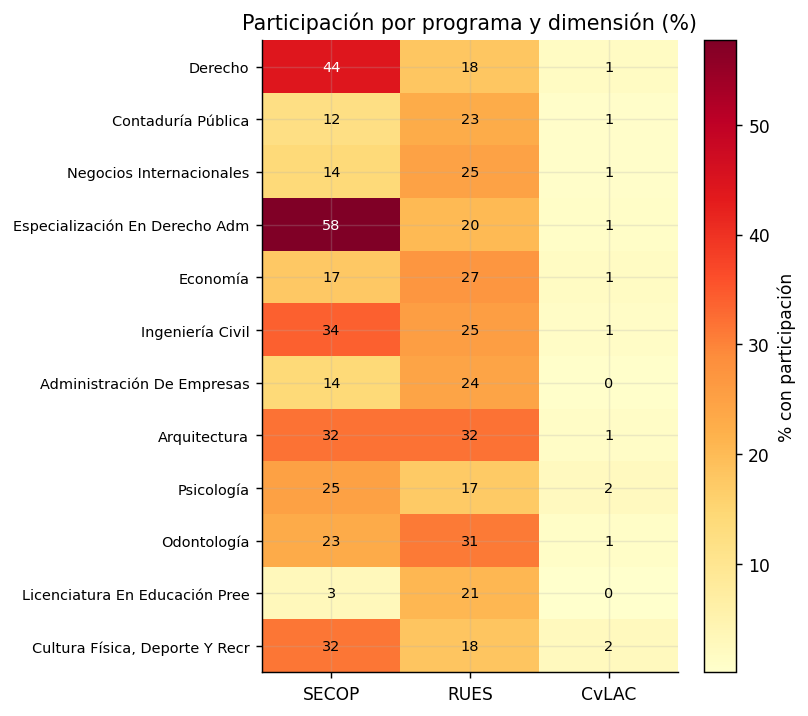
\includegraphics[width=0.66\linewidth]{figs_cruce/16_heatmap_programa.png}\caption{Mapa de calor de tasas de participación por programa y dimensión.}\label{fig:heatmap-programa}\end{figure}

Los programas jurídicos lideran la contratación pública: la Especialización en Derecho Administrativo alcanza el 57,7\,\% de sus graduados en SECOP y el Derecho el 44,1\,\%, seguidos de la Ingeniería Civil y la Arquitectura, disciplinas cuyo ejercicio gravita hacia el sector público. El registro empresarial se concentra en cambio en programas del área económica, del hábitat y de la salud, con Arquitectura (32,0\,\%), Odontología (31,1\,\%) y Economía (27,0\,\%) a la cabeza. La trayectoria investigativa, siempre minoritaria, es algo más visible en Cultura Física, Deporte y Recreación (2,4\,\%), Psicología (2,3\,\%) y Derecho (1,5\,\%). Programas de marcada vocación docente, como la Licenciatura en Educación Preescolar y Promoción de la Familia, muestran tasas bajas en las tres dimensiones, señal de que su participación se ejerce por canales ---la docencia, el aula--- que estas fuentes públicas no capturan. El cruce por programa convierte así el dato agregado en una herramienta de gestión curricular, al mostrar a cada facultad la vocación de participación predominante de sus egresados y, con ella, las dimensiones donde conviene reforzar el acompañamiento.

\begin{cajahallazgo}
El egresado tomasino deja huella sobre todo en una dimensión, pero existe un núcleo multidimensional que combina dos o las tres facetas: 12.149 graduados reúnen dos dimensiones y 227 las tres. Esa densidad crece con el posgrado y se concentra en Tunja, y la asociación entre contratación, matrícula mercantil e investigación reconocida ---en particular la presencia de los investigadores también en SECOP y RUES--- sugiere que estas formas de participación tienden a acompañarse antes que a excluirse. Se trata de una asociación y no de una relación causal, pero es justamente la convergencia que ninguna fuente aislada podía ver y que el Observatorio de Participación de Graduados pone por primera vez a la vista.
\end{cajahallazgo}
